%% You can use this file to create your answer for Exercise 1.  
%% Fill in the places labeled by comments.
%% Generate a PDF document by with the command `pdflatex ex1'.

\documentclass[11pt]{article}


\usepackage{times}
\usepackage{listings}
\usepackage{enumerate}
\usepackage{courier}
\usepackage{hyperref}
\usepackage{xcolor}
\usepackage{graphicx}

%% Values that are specific to a particular term
\newcommand{\thisterm}{Spring 2021}

\newcommand{\dateassigned}{Fri.,~Feb.~5}

%% Printed form of home page that students should use
\newcommand{\visiblecoursehome}{http://www.cs.cmu.edu/\textasciitilde{}418}

%% Link to home page that will stay valid
\newcommand{\actualcoursehome}{http://www.cs.cmu.edu/afs/cs.cmu.edu/academic/class/15418-s21/www}

\newcommand{\datedueregistered}{Wed.,~Feb.~17}
\newcommand{\dateduewaitlist}{Wed.,~Feb..~17}




%% Page layout
\oddsidemargin 0pt
\evensidemargin 0pt
\textheight 600pt
\textwidth 469pt
\setlength{\parindent}{0em}
\setlength{\parskip}{1ex}

%% Colored hyperlink 
\newcommand{\cref}[2]{\href{#1}{\color{blue}#2}}

%% Customization to listing
\lstset{basicstyle=\ttfamily,language=C++,morekeywords={uniform,foreach}}

%% Enumerate environment with alphabetic labels
\newenvironment{choice}{\begin{enumerate}[A.]}{\end{enumerate}}
%% Environment for supplying answers to problem
\newenvironment{answer}{\begin{minipage}[c][1.5in]{\textwidth}}{\end{minipage}}
\newenvironment{answer2}{\begin{minipage}[c][0.5in]{\textwidth}}{\end{minipage}}

\begin{document}
\begin{flushright}
{\large\bf Full Name: \makebox[2in][l]{
%% Put your name on the next line

}} \\[1ex]

{\large\bf Andrew Id: \makebox[2in][l]{\tt
%% Put your Andrew ID on the next line

}} \\[1ex]
\end{flushright}
\vspace*{0.3in}
\begin{center}
\LARGE
15-418/618 \thisterm{} \\
Exercise 1
\\ 
\end{center}

\begin{center}
\Large
\begin{tabular}{lll}
\hline
 & Registered students & Waitlist students \\
\hline
Assigned: & \dateassigned{} & \dateassigned{} \\
Due: &  \datedueregistered{}, 11:00~pm & \dateduewaitlist{}, 11:00~pm \\
\hline
\end{tabular}
\end{center}

\section*{Overview}

This exercise is designed to help you better understand the lecture
material and be prepared for the style of questions you will get on
the exams.  The questions are designed to have simple answers.  Any
explanation you provide can be brief---at most 3 sentences.
You should work on this on your own, since that's how things will be when
you take an exam.

You will submit an electronic version of this assignment to Canvas as
a PDF file.  For those of you familiar with the \LaTeX{} text formatter, you can download the template and configuration files at:
\begin{center}
  \cref{\actualcoursehome/exercises/ex1.zip}{\visiblecoursehome/exercises/ex1.zip}\\
%   \cref{\actualcoursehome/exercises/ex1.tex}{\visiblecoursehome/exercises/ex1.tex}
\end{center}
Instructions for how to use this template are included as comments in the file.  Otherwise,
you can use this PDF document as your starting point.
You can either: 1) electronically modify the PDF, or 2) print it
out, write your answers by hand, and scan it.  In any case, we expect
your solution to follow the formatting of this document.

\newpage

\section*{Problem 1: Instruction-Level Parallelism}

Consider the following code where each line within the function
represents a single instruction.
\begin{lstlisting}
typedef struct {
    float x;
    float y;
} point;

inline void innerProduct(point *a, point *b, float *result)
{
    float x1 = a->x; // Uses a load instruction
    float x2 = b->x;
    float product1 = x1*x2;
    float y1 = a->y;
    float y2 = b->y;
    float product2 = y1*y2;
    float inner = product1 + product2;
    *result = inner; // Uses a store instruction
}

void computeInnerProduct(point A[], point B[], float result[], int N)
{
    for (int i = 0; i < N; i++)
        innerProduct(&A[i], &B[i], &result[i]);
}
\end{lstlisting}

In the following questions,
you can assume the following:
\begin{itemize}
\item $N$ is very large ($> 10^6$).
\item The machines described have modern CPUs, providing
out-of-order execution, speculative execution, branch prediction, etc.
\begin{itemize}
\item There are ample resources for fetching, decoding, and committing instructions.  The only performance limitations are due to
the number, capabilities, and latencies of the execution units.
\item The branch prediction is perfect.
\end{itemize}
\item There are no cache misses.
\item The overhead of updating
the loop index {\tt i} is negligible.
\item The load/store units perform any necessary address arithmetic.
\item The overhead due to procedure calls, as well as starting and ending loops, is negligible.
\end{itemize}

\newpage

Suppose you have a machine $M_1$ with two load/store units
  that can each load or store a single value on each clock cycle, and
  one arithmetic unit that can perform one arithmetic operation
  (e.g., multiplication or addition) on each clock cycle.


\begin{choice}
\item  
Assume that the load/store and arithmetic units have latencies of one cycle.
How many clock cycles would be required to
execute \texttt{computeInnerProduct} as a function of $N$?    Explain what limits the performance.

\begin{answer}
  It takes $6N$ clock cycles since x1,x2 and y1,y2 loads together. Data dependencies limits the parallelism in this function.
\end{answer}
\item
Now assume that the load/store and arithmetic unit have
latencies of 10 clock cycles, but they are fully pipelined, able to
initiate new operations every clock cycle.  
How many clock cycles would be required to
execute \texttt{computeInnerProduct} as a function of $N$?    Explain how this relates to your answer to part A.

\begin{answer}
x1,x2 takes 10 cycle. Y1,y2 takes 10 cycle. Product2, inner result takes each 10 cycle. Total of 50 cycle. This time calculation of product1 is not visible to programmer.
\end{answer}
\end{choice}

\newpage

\section*{Problem 2: A Yinzer Processor Pipeline}

Yinzer Processors builds a single core, single threaded processor that executes instructions using a simple four-stage pipeline. As shown in the figure below, each unit performs its work for an instruction \textbf{in one clock}. To keep things simple, assume this is the case for all instructions in the program, including loads and stores (memory is infinitely fast).\\
The figure shows the execution of a program with six \textbf{independent instructions} on this processor. \textit{However, if instruction B depends on the results of instruction A, instruction B will not begin the IF phase of execution until the clock after WB completes for A.}

\begin{center}
    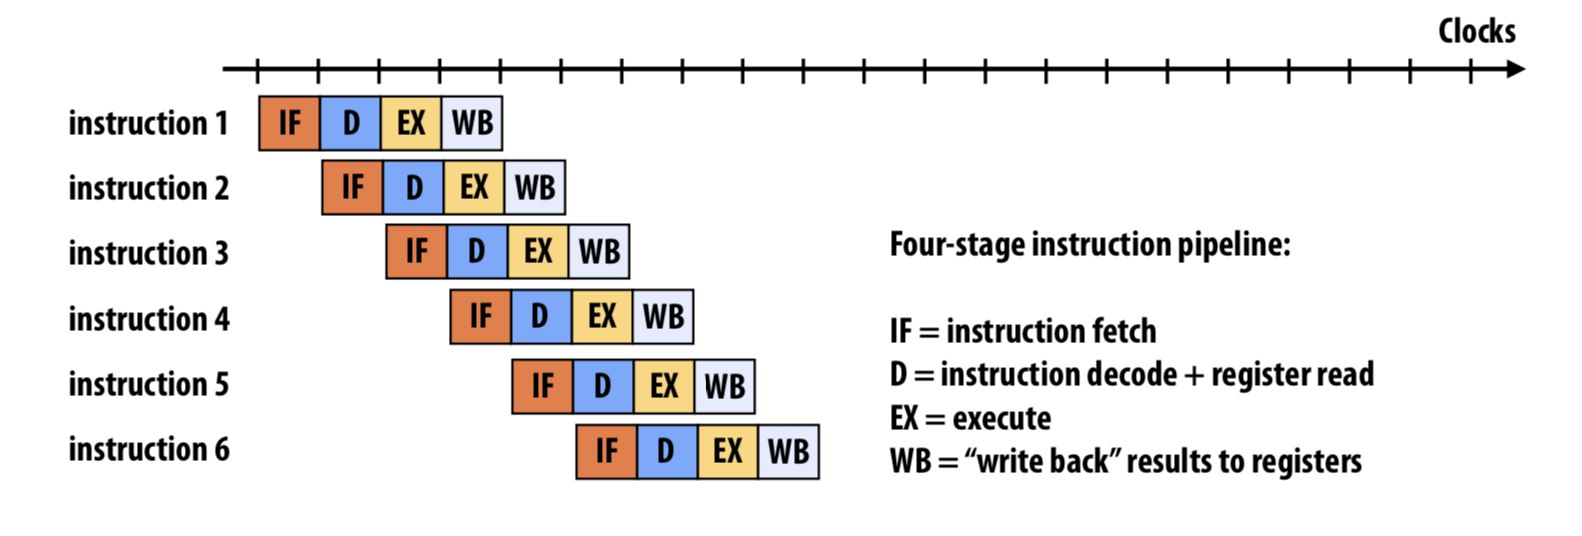
\includegraphics[width = 450px]{yinzer.png}\\
\end{center}



\begin{choice}
\item  
Assuming all instructions in a program are \textbf{independent} (yes, a bit unrealistic) what is the instruction throughput of the processor?

\begin{answer2}
$N$ program takes $3+N$ cycle.
\end{answer2}
\item
Assuming all instructions in a program are \textbf{dependent} on the previous instruction, what is the instruction throughput of the processor?

\begin{answer2}
$N$ program takes $(4+1)*N$ cycle.
\end{answer2}
\item What is the latency of completing an instruction?

\begin{answer2}
1 clock cycle because WB \textvisiblespace IF
\end{answer2}
\item Imagine the EX stage is modified to improve its throughput to two instructions per clock. What is the new overall maximum instruction throughput of the processor for independent instructions?

\begin{answer2}
It does not change because the critical path stays still.
\end{answer2}

\end{choice}

\end{document}
